\section{Εισαγωγή}
\selectlanguage{greek}
Ένα μεμονωμένο μυρμήγκι δεν μπορεί να κάνει πολλά, τα μυρμήγκια ως σύνολο όμως, όπως και κάθε άλλο είδος εντόμων που λειτουργούν ομαδικά ως σμήνος για την επίτευξη κοινού στόχου, μπορούν να ολοκληρώσουν εξειδικευμένες εργασίες γρήγορα και αποτελεσματικά. Αυτό αποτελεί πηγή έμπνευσης για τον αλγόριθμο που θα μελετήσουμε σε αυτήν την εργασία καθώς και για πολλούς άλλους αλγόριθμους σμήνους που έχουν ως στόχο την επίλυση πολύπλοκων προβλημάτων βελτιστοποίησης πραγματικού κόσμου \cite{dorigo2004ant}. 

Τα τελευταία χρόνια, τέτοια προβλήματα παρουσιάζονται σε διάφορους κλάδους με πλη- θώρα θεωρητικών και πρακτικών εφαρμογών όπως το πρόβλημα γεφυρών και το πρόβλημα του πλανόδιου πωλητή (\lt{Travelling Salesman Problem - TSP}) καθώς και σε κοινωνικά δίκτυα, δίκτυα δρομολόγησης \cite{gkertsis2023thewria}, προβλήματα προσβασιμότητας, βελτιστοποίηση δικτύων επικοινωνίας, σχεδίαση ηλεκτρικών κυκλωμάτων, και άλλα, για το λόγο αυτό, ιδιαίτερο ε- νδιαφέρον έχει αναπτυχθεί για την μελέτη τους \cite{manwlopoulos2014thewria}.

Ο αλγόριθμος της αποικίας μυρμηγκιών (\lt{Ant Colony Optimisation - ACO}) που θα αναλυθεί στην παρούσα πτυχιακή εργασία είναι ένας αλγόριθμος νοημοσύνης σμήνους και με χρήση αυτού αντιμετωπίζονται τέτοια προβλήματα. Ο όρος "Νοημοσύνη Σμήνους" (\lt{swarm intelligence}) πρωτοεμφανίστηκε το 1989 από τους \lt{Gerardo Beni} και \lt{Jing Wang} \cite{10.1007/978-3-642-58069-7_38} και μας βοηθάνε στην επίλυση προβλημάτων βελτιστοποίησης, ενώ το 1992 προτάθηκε ο \lt{ACO} μέσω της διδακτορικής διατριβής του \lt{Marco Dorigo}. Οι αλγόριθμοι αυτοί μιμούνται εξελικτικές διαδικασίες που παρουσιάζονται στην φύση όπως η επιλογή μιας διαδρομής και η προσαρμογή σε νέα δεδομένα. Ο αλγόριθμος της αποικίας των μυρμηγκιών συγκεκριμένα βασίζεται, όπως προκύπτει κι από το όνομα του, στη συμπεριφορά των μυρμηγκιών στην φύση και το πώς καταφέρνουν πάντα να βρίσκουν την βέλτιστη διαδρομή σε όποιο πρόβλημα τους παρουσιαστεί με χρήση πιθανολογικών τεχνικών. Πέρα από τον \lt{ACO}, παραδείγματα άλλων τέτοιων αλγορίθμων είναι ο αλγόριθμος βελτιστοποίησης σμήνους σωματιδίων (\lt{Particle Swarm Optimisation - PSO}), ο αλγόριθμος των μελισσών (\lt{Artificial Bee Colony Algorithm - ABC}), οι διάφοροι γενετικοί αλγόριθμοι (\lt{Genetic Algorithms- GA}) και πολλοί άλλοι \cite{mavrovouniotis2017survey}.

Ένα κεφάλαιο απαραίτητο για την υλοποίηση αυτού του αλγόριθμου είναι η θεωρία γράφων. Έννοιες στις οποίες βασίζεται ο \lt{ACO} όπως η φερομόνη (\lt{pheromone}) και το κόστος διαδρομής (\lt{cost}), μοντελοποιούνται με χρήση αυτής. Κάθε ακμή (\lt{edge}) του γράφου αντιστοιχεί σε μία τιμή φερομόνης, η οποία ανανεώνεται καθώς τα μυρμήγκια περνούν από αυτήν. Τα μυρμήγκια εξερευνούν πιθανές διαδρομές, και ενισχύουν την ποσότητα φερομόνης στις καλύτερες, επηρεάζοντας έτσι τις επιλογές των μυρμηγκιών που ακολουθούν δίνοντας στον αλγόριθμο την δυνατότητα να "θυμάται" προηγούμενες λύσεις και να τις αξιοποιεί στο μέλλον. 


\begin{flushright} 
    \lt{I am lost! Where is the line?!
    
    —A Bug’s Life, Walt Disney, 1998}\cite{dorigo2004ant}
\end{flushright}

\subsection{Ιστορική Αναδρομή}
\begin{figure}[ht]
    \begin{minipage}[c]{.46\linewidth}
        \centering
        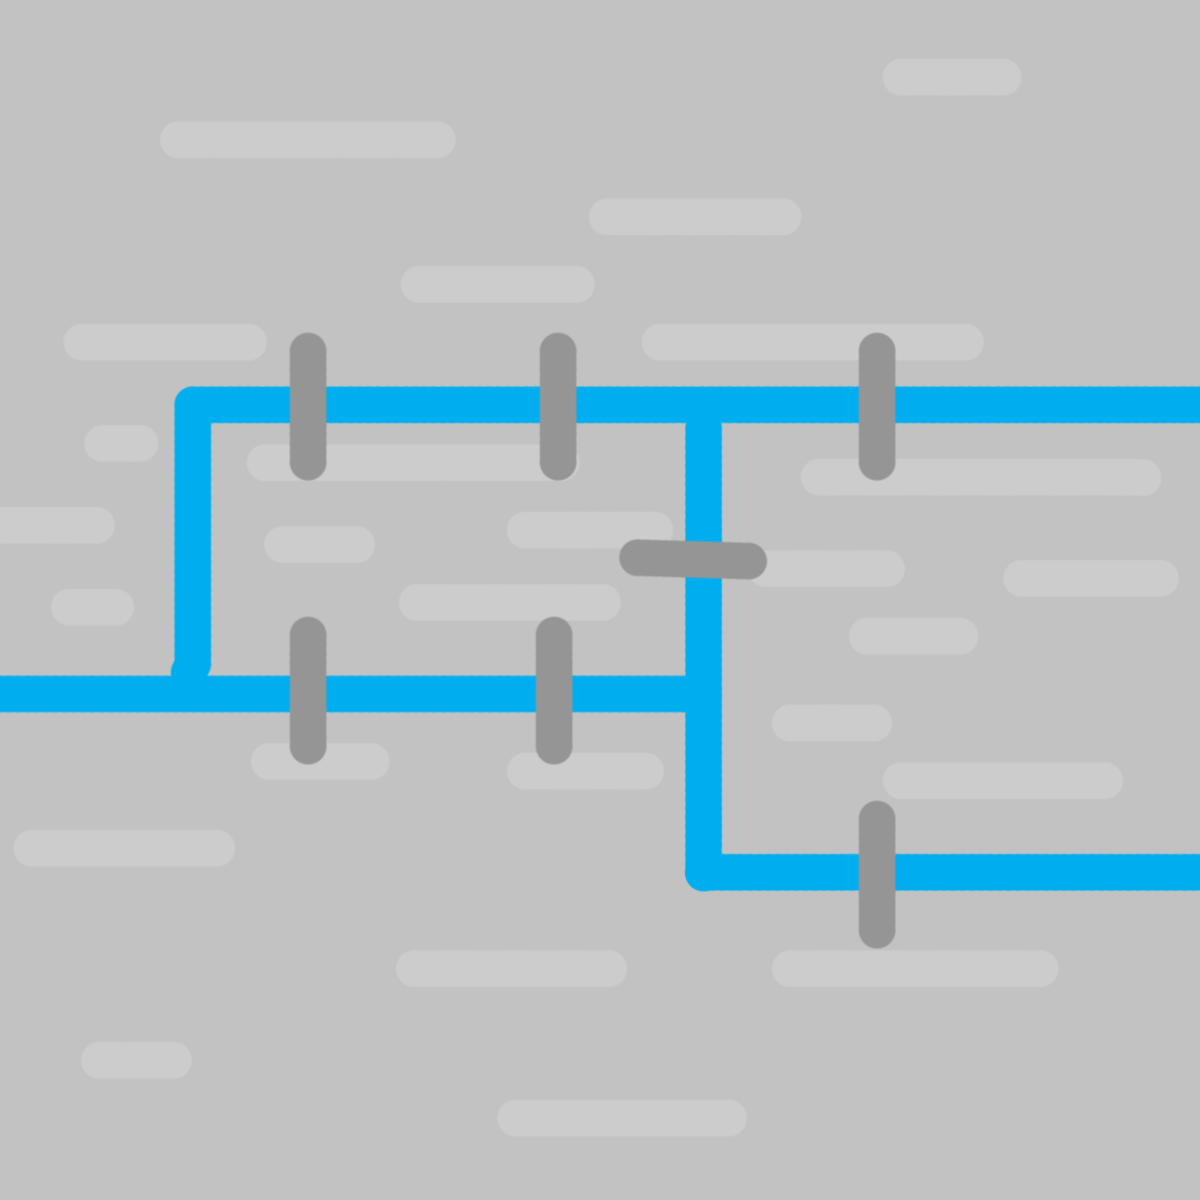
\includegraphics[scale=0.15]{2947_thesis/pictures/konigsberg.png}
        \caption{Προσομοίωση Königsberg.}
        \label{1}
    \end{minipage}
    \hfill%
    \begin{minipage}[c]{.46\linewidth}
        \centering
        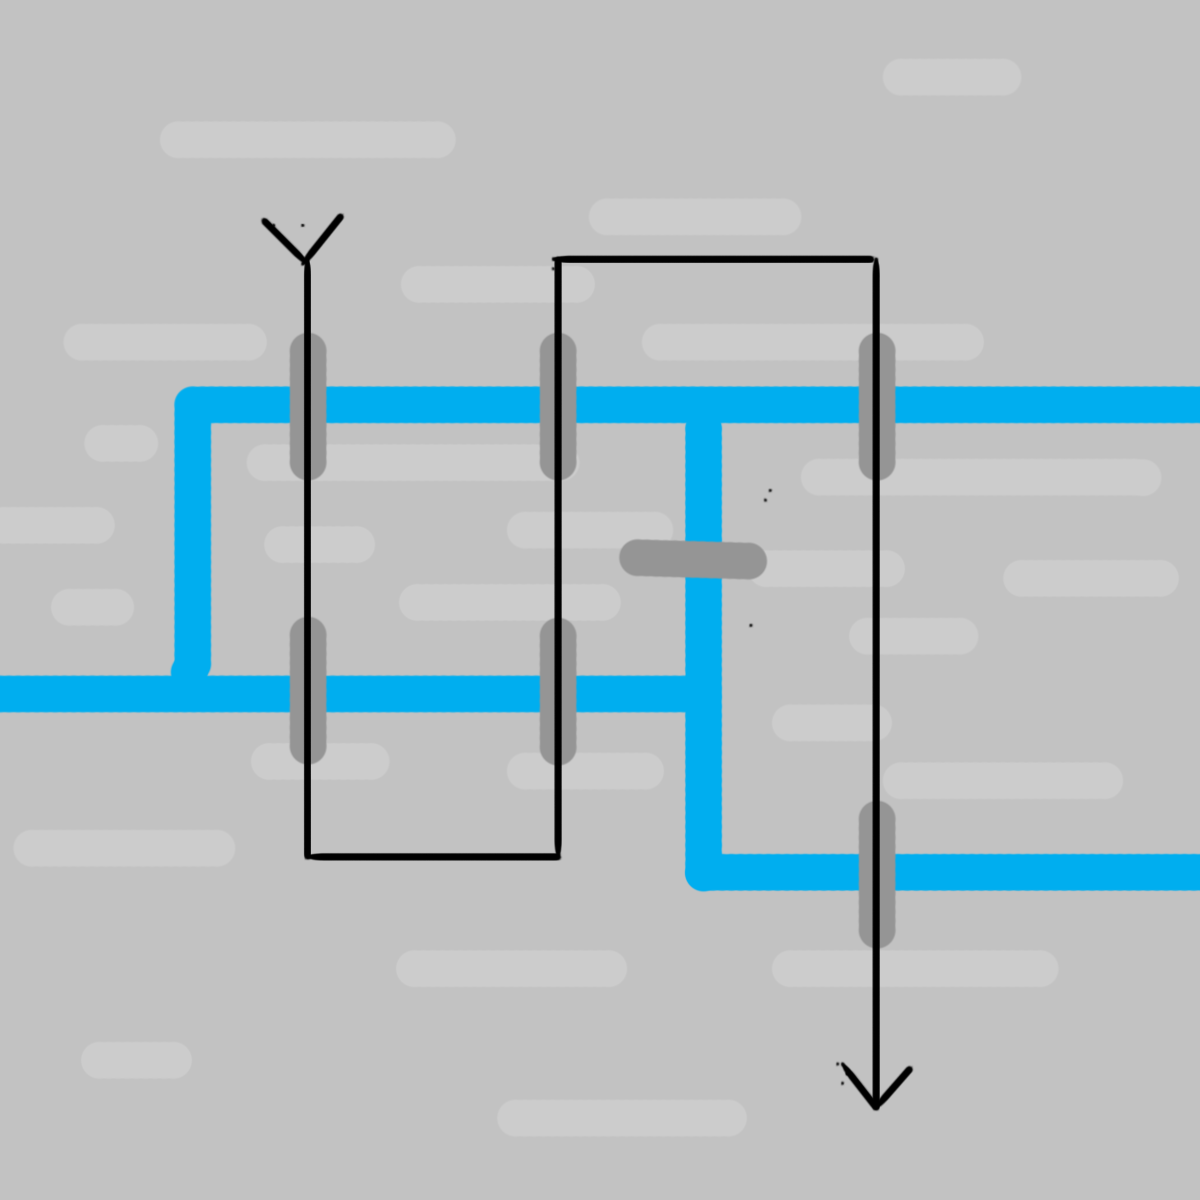
\includegraphics[scale=0.15]{2947_thesis/pictures/konigsbergEx.png} 
        \caption{Παράδειγμα διάσχισης γεφυρών}
        \label{2}
    \end{minipage}
\end{figure}
Η ανάπτυξη της θεωρίας γράφων (\lt{graph theory}) ξεκίνησε τον 18ο αιώνα και πιο συγκεκριμένα το 1736 στην πόλη \lt{Königsberg} της Πρωσίας. Σήμερα είναι το Ρωσικό \lt{Kaliningrad} (μεταξύ Λιθουανίας και Πολωνίας στη Βαλτική) \cite{manwlopoulos2014thewria}. Η πόλη ήταν χωρισμένη σε 4 τμήματα από τον ποταμό \lt{Pregel} και χρησιμοποιούνταν 7 γέφυρες για να γίνεται εφικτή η διέλευση των κατοίκων στα διάφορα τμήματά της εικόνας \ref{1}. Όταν ο Ελβετός μαθηματικός \lt{Leonard Euler} αναρωτήθηκε αν είναι εφικτό να διασχίσει κάποιος τις γέφυρες της πόλης με βασικό περιορισμό να διασχιστούν όλες οι γέφυρες μόνο μία φορά (Πρόβλημα των 7 γεφυρών του \lt{Königsberg}) \ref{2}, ένας νέος κλάδος των διακριτών μαθηματικών γεννήθηκε, γνωστός και ως θεωρία γράφων. Ο \lt{Euler} απέδειξε ότι δεν υπάρχει τέτοια διαδρομή μέσω της χρήσης γράφων \lt{Graph Theory} και κατά συνέπεια το πρόβλημα δεν έχει λύση. Αυτή η απόδειξη απέκτησε αξία όταν ο \lt{Euler} την εφάρμοσε και σε άλλα προβλήματα γράφων και γενίκευσε την βασική ιδέα. 

Ένα μονοπάτι (\lt{path}) ονομάζεται μονοπάτι \lt{Euler (Eulerian path} ή \lt{Eulerian trail}) όταν μπορούμε να επισκεφτούμε κάθε περιοχή-κορυφή (\lt{vertice}) διασχίζοντας την κάθε γέφυρα-ακμή (\lt{edge}) μόνο μία φορά (και ονομάζεται κυκλική αν καταλήγουμε εκεί που ξεκινήσαμε), αν υπάρχει ένα τέτοιο μονοπάτι σε ένα γράφο τότε αυτός ο γράφος ονομάζεται γράφος \lt{Euler} (\lt{Eulerian graph}) \cite{ntenisiwtis2023thewria}. Στο σχήμα \ref{3} που αντιπροσωπεύει την πόλη του \lt{Königsberg} σε μορφή γράφου δεν υπάρχει μια τέτοια διαδρομή. Για να γίνει αυτό πρέπει να αφαιρέσουμε μία γέφυρα-ακμή όπως φαίνεται στο σσχήμα \ref{4}. Αποδείχθηκε από τον \lt{Euler} ότι όλες οι κορυφές πρέπει να έχουν άρτιο πλήθος ακμών που προσπίπτουν σε αυτή την κορυφή (βαθμό - \lt{degree}), εκτός από αυτές  που ξεκινά και τελειώνει η διαδρομή, εκτός κι αν η διαδρομή είναι κυκλική. Πιο συγκεκριμένα, ένας συνδεδεμένος γράφος $Graph(Vertices,Edges)$ είναι γράφος Euler αν και μόνο αν δεν έχει κορυφές (\lt{vertices}) περιττού βαθμού \cite{bondy1976usr}.